\section{Experiment 2}
\subsection{Methodology} \label{method-2}

%<---------------------------->%
% Motivation
%% The second experiment takes a step futher
%%% First: Mimics an HCI setting (generalization)
%%% Second: Different perspective
%%% Third: Different impact setting
%% We created a HCI scenerio and measure participant's preference using Likert, QV and a monetary task.
%<---------------------------->%

The first experiment results demonstrated strong implication that QV aligns closer to the participant's real preference compared to the Likert scale when choosing among a spectrum of societal issues. To take a step further, we designed the second experiment with three different changes compared to the previous experiment. These three changes will allow us to understand QV's generalizability across different application domains. First, we changed the application domain form societal causes to an HCI application. Second, this experiment focused on items on the ballot that are of different \textit{perspectives} for the same subject matter, rather than having different \textit{options} contributing to the same topic as we did in the first experiment. Recall we asked participants to choose among different societal causes (items) that impacted the society as a whole (topic). This subtle difference lies in the different \textit{relationships} between the items on the ballot. To give a simple analogy: if the first experiment asked about one's preference among chocolate, strawberry, and vanilla ice cream (options), the second experiment asked how much does one care about the texture, flavor, and color of ice cream (perspectives). Third, the second experiment focused on settings that survey short-term and more immediate outcomes compared to a more abstract and further-in-the-future impact. Many market research studies customer's experience with their product compared to governments that poll for people's opinions on mid to long term societal causes. In experiment two, we changed the topic domain of the survey, elected different items to put on the ballot, and chose a more immediate-impact setting. We hypothesis that QV will still outperform Likert at presenting the subject's true preferences. 

To test our hypothesis, we designed a between within-subject study with two groups of participants. Both groups of participants completed an HCI study using different measuring techniques. In this section, we first explain the HCI study scenario we designed, followed by the experiment workflow accompanied by details and interface of the experiment design.

%<---------------------------->%
% HCI Experiment background
%% Video HCI experiments
%% Selection of the five elements and their definitions
%% The goal of this HCI experiment is to find elements that impact participants most.
%<---------------------------->%
 
\subsection{Choice of HCI study}
It is crucial for us to design an HCI study scenario that aligns with the three focuses proposed in the previous subsection. On top of that, we also want to avoid creating an entire new HCI study that requires sophisticated verification. Most HCI researchers used Likert surveys to understand the participants' opinions across one or more devices, designs, or interfaces. However, reproducing one of these experiences can be costly and difficult because of the availability of these devices, designs, or interfaces.

We want a well-explored HCI topic that we could rely on and still maintain ecological validity. Therefore, we turn to the other typical use case where UX/UI researchers aimed to prioritize features and elements that their customers care about. We often see these forms as online feedback forms, for example, asking users to rate the design, friendliness, helpfulness, and content quality of a chatbot.

We created a video playback experience HCI research scenario for this experiment. Research on video and audio elements of video playback from the lens of HCI has been relatively mature. Researchers provided insights to fields like multi-media conferencing \cite{watson1996evaluating}, video-audio perception \cite{chen2006cognitive, molnar2015assessing}and more specifically trade-offs between video and audio elements under network-monetary constraints \cite{molnar2013comedy, oeldorf2012bad}. \textcite{oeldorf2012bad}, for example, conducted a study to understand how users with bandwidth constraints made trade-offs covering a broad set of elements across multiple videos and audio elements. They examined participants' attitudes between three video bit rates, three video frame rates, and two audio sampling rates across three types of video content. Participants rated the overall quality, video quality, audio quality, and enjoyment level on a 5-point Likert scale in each condition. The study derived the conclusion from the mean and standard deviation of the survey results. This is a typical study to locate one or some of the $K$ elements to choose from when under constraint.

We mimic this experiment and propose a similar user research scenario that tries to answer the following question: ``Given limited bandwidth, how important do participants think the five video and audio elements were to a video watching experience?'' Based on related works, we elected five video playback elements: (1) Stability of Video Imagery \cite{claypool1999effects}, (2) Stability of Audio \cite{claypool1999effects}, (3) Quality of audio \cite{oeldorf2012bad, noll1993wideband}, (4) Quality of the video \cite{oeldorf2012bad, knoche2008low}, and (5) Audio-Video Synchronization \cite{steinmetz1996human}. The ``Stability of Video Imagery'' refers to how smooth the visuals of the video plays. Lost packets during playback causes froze frames. The more lost packets, the more staggered the video seems. The ``Stability of Audio'' is similar to ``Stability of Video Imagery'', which refers to the smoothness the audio is. Lost audio packets create silence, causing the audio to stutter. The ``Quality of audio'' refers to how clear and crisp the sound quality is of the video. With a lower audio sampling rate, the playback required a smaller audio file and vice versa. The lower the audio quality, the more muffled and unclear the audio sounds. Similar to audio quality, the ``Quality of the video'' refers to how sharp the visuals in the video are. Resolutions are proportion to the number of pixels sent to the client from the server. Hence, by altering the length and width of the video, or pixel density per inch, we change the video file's quality and size. The smaller the pixels, the more pixelated and unclear the video seems. Finally, the ``Video-audio Synchronization'' is how well video visuals synchronized with the audio playback. In our experiment, we focus on having audio play ahead of the video only.

Since there are no previous studies that looked at the combination of all these video elements, we make use of individual studies to decide the value associated with the different levels of changes for each of these elements. In short, we use a video-audio experiment that aims to find video/audio factors that impact participants the most to test the performance between Likert and QV.


\begin{figure}[htpb]
    \centering
    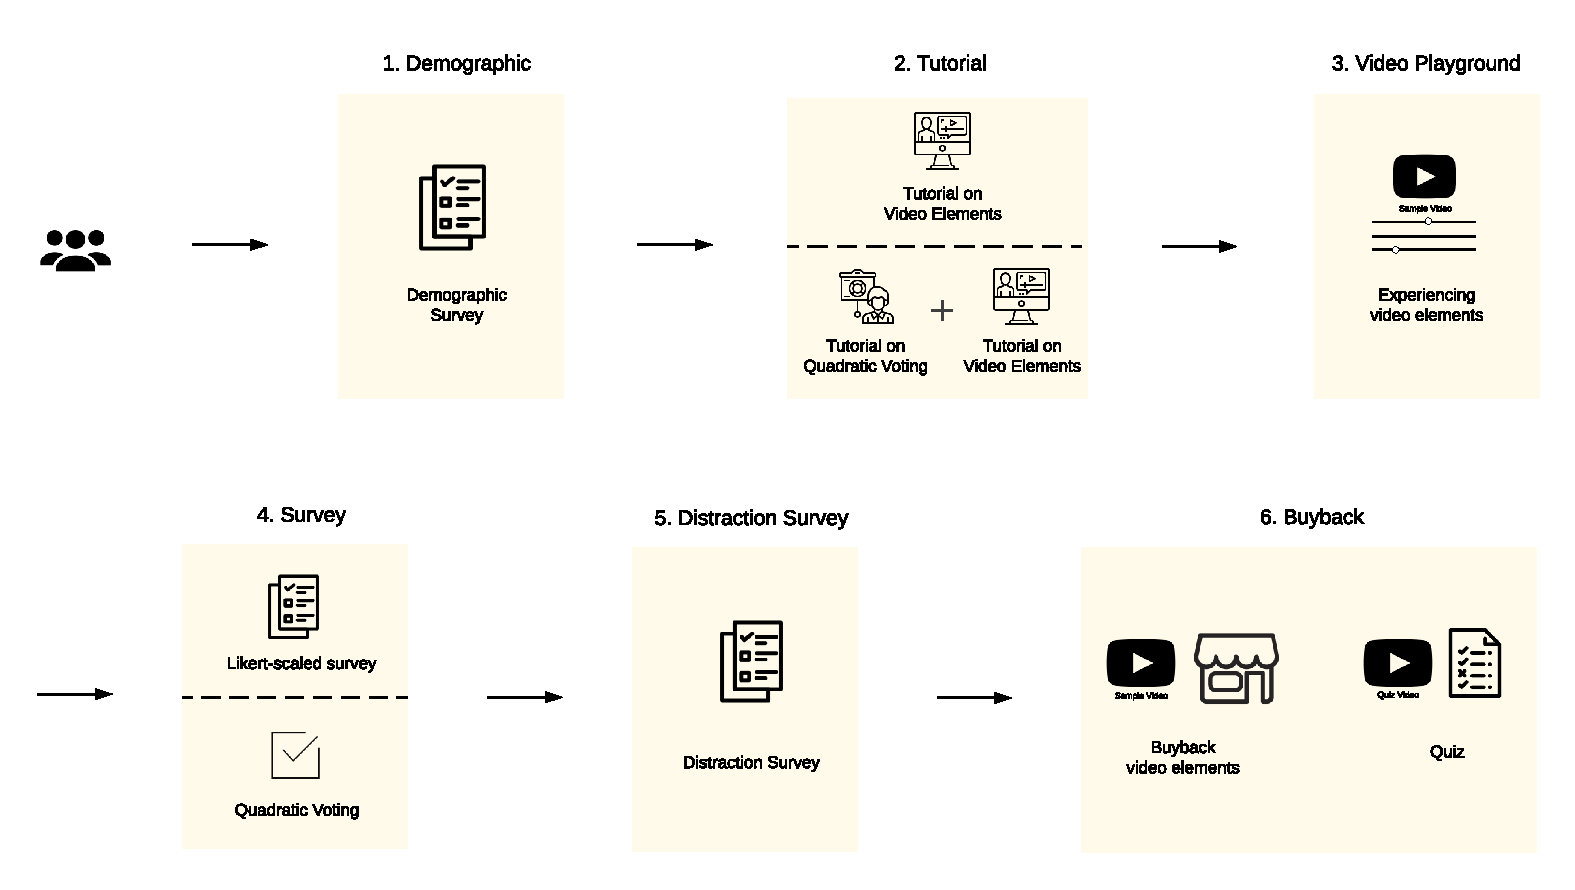
\includegraphics[width=\textwidth, keepaspectratio=true]{content/image/new_exp2_flow.pdf}
    \caption{
        Experiment two is conducted between within subject. There are two groups of participants. Participants would go through five steps. Steps with dashed lines indicated difference among the two groups. The one on top is the likert group while the one on the bottom is the QV group.
    }
    \label{fig:exp2_flow}
\end{figure}

\subsection{Experiment Flow}

We recruited 180 participants through MTurk. To compare how Likert survey and QV reflects people's underlying preferences, we desgined the following experiment. All participants followed five steps, the shaded area in Figure \ref{fig:exp2_flow}, starting with (1) Demographics, (2) Learning and attention checks, (3) Video Playground, (4) Expressing attitude, and (5) The buyback task. We divided participants equally into two groups: Likert and QV. Now we explain the five steps in detail.

\subsubsection{Step 1. Demographic}
We greet participants with a consent form. In the cosnent form, we pitched ourself as researchers from an airline online video streaming service. We told the participants that we want to collect people's thoughts across differernt video playback elements. We did not tell the participants that this experiment aims to compare Likert and QV until the participants completed the experiment. Once participants accepted the consent form, participants will fill out a demographic survey. This demographic survey is identical to the first experiment.

\subsubsection{Step 2. Learning and attention checks}
In the second step, we provided both groups of participants with a tutorial on the definition of the five different video elements of video-playback. These five elements were described in the previous subsection. Once participants think they understood the concepts, we asked participants to answer five mutiple choice questions. Participants that failed to answer four out of five questions correctly will be qisquality to compelte the experiment. This assured that participants fully understood the terminology used in the experiment and are taking the experiment seriously. Given that QV to be unpopular among the mass, we added an additional tutorial on QV and attention checks specific to QV for the QV Group. This tutorial is similiar to the one in experiment one where we provided a QV video tutorial and a QV playgorund for participants to play with. The quiz consists of five true false question. Participants that answered two or more incorrectly will be disqualified to compelte the experiment.

\begin{figure}[htpb]
    \centering
    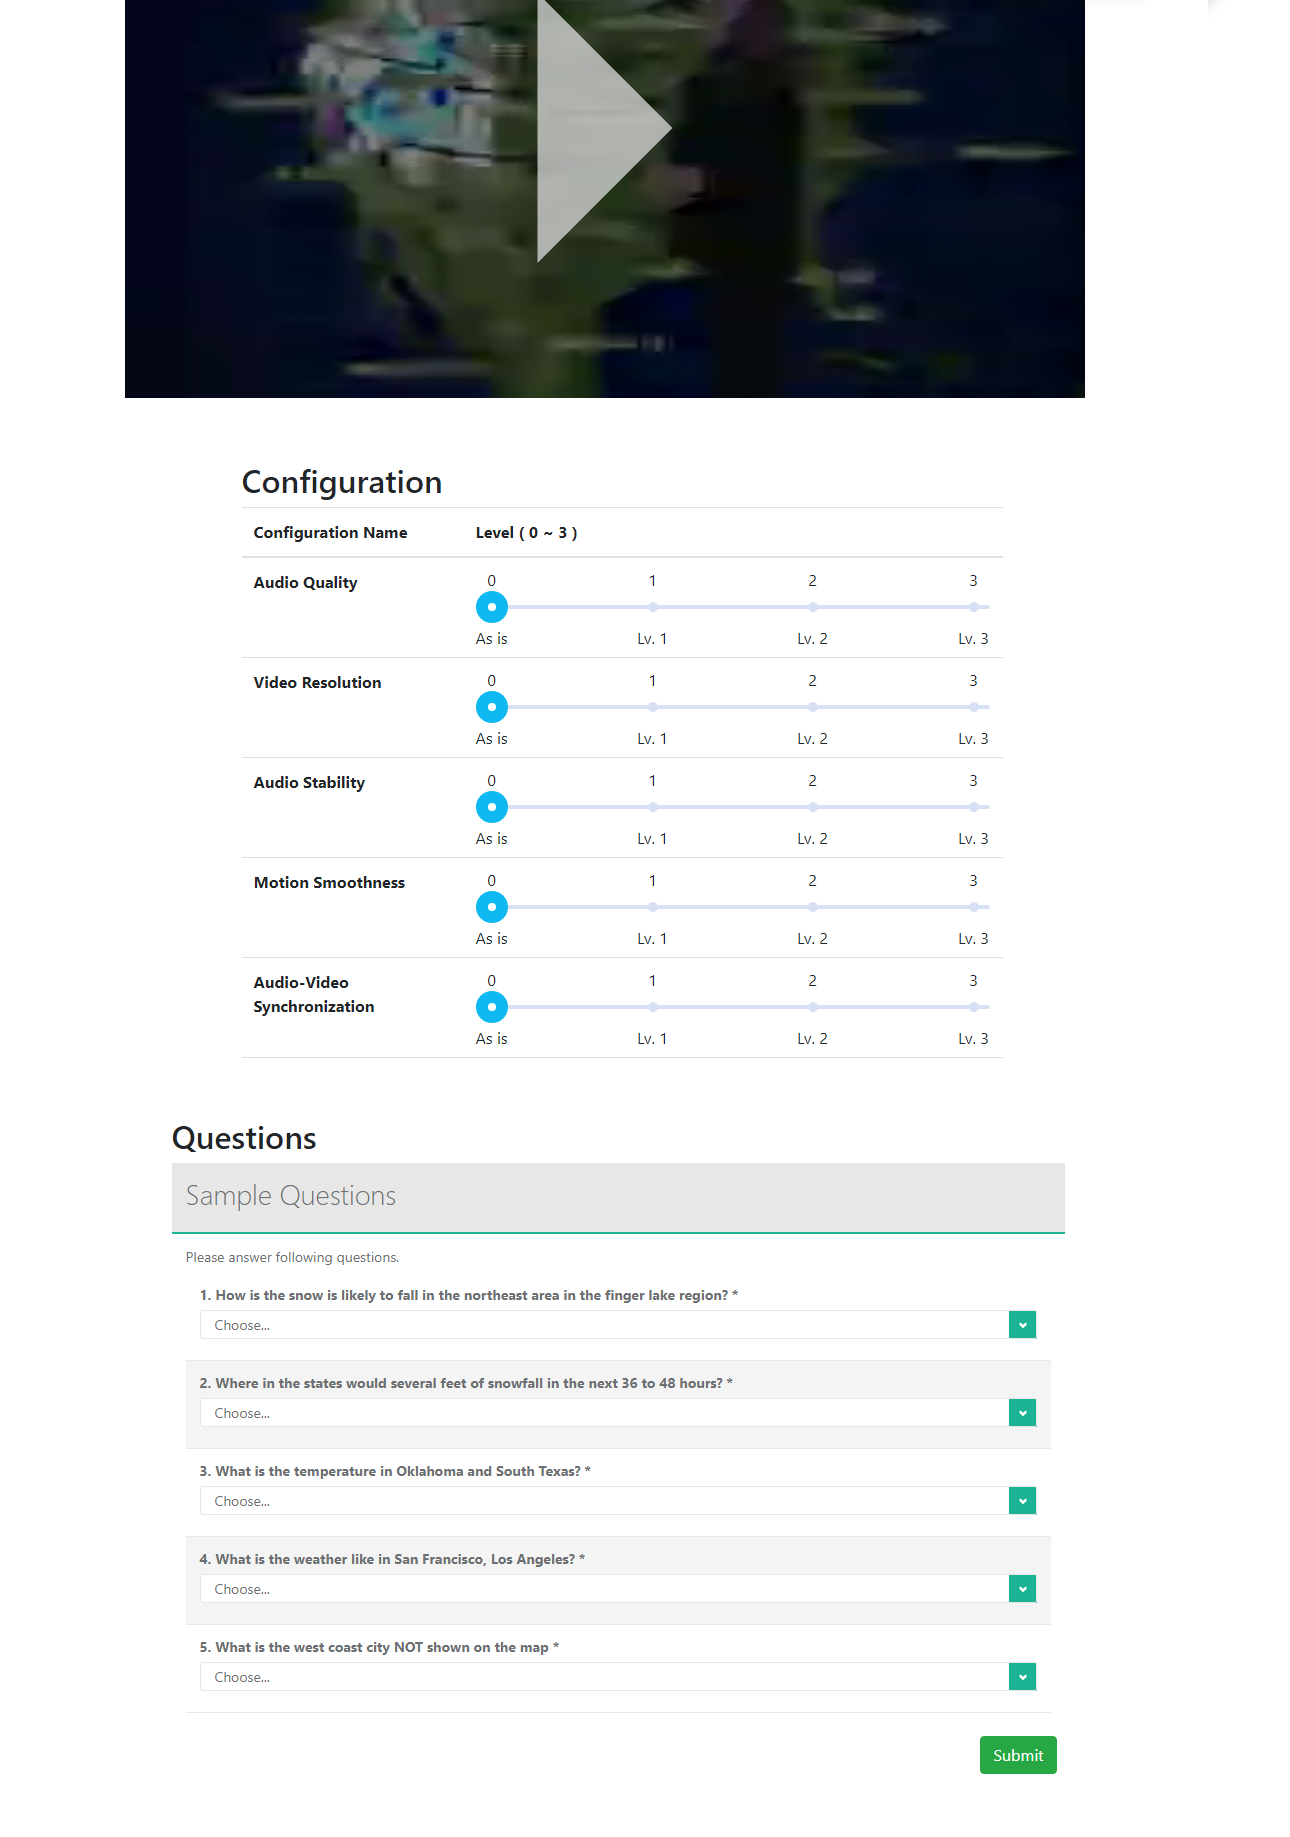
\includegraphics[width=\textwidth, keepaspectratio=true]{content/image/exp2_playground.png}
    \caption{
        The Real-time Video Element Interface allows participants to play and understand how different levels of video playback element impacts their viewing experience. Participants were asked to complete the five mutiple choice questions relevent to the video content.
    }
    \label{fig:exp2_playground}
\end{figure}


\subsubsection{Step 3. Video Playground}
Once participants passed the attention checks, we reminded them that our goal is to learn about their preferences in valuing different video elements during video playback. To help them understand better, we built a video playground shown in Fig \ref{fig:exp2_playground}. This playground will provide them a playground that allows hands-on experience on different combinations of the different levels of the various video elements that impact their viewing experiences.

This interface showcased a weather video on top of the page. For each of the five video playback elements, we provided a sidebar that had four levels of toggles. Participants can toggle any of these five elements to any of the four levels at any time. According to the setting participant's set, the video playback will immediately apply those changes. Participants can pause and play the video at any time, and they can reply to the video as many times as they like. We expect participants to test out different combinations freely in this playground.

We made use of past research to decide the changes between each toggle. The four levels of the five video playback elements are listed below:
\begin{itemize}
    %20\%, 8\%, 4\%, and 0\%
    \item Stability of Video Imagery: 30\%, 12\%, 2\%, and 0\%
    %20\%, 8\%, 4\%, and 0\%
    \item Stability of Audio: 30\%, 12\%, 2\%, and 0\%
    %8kHz, 11kHz, 16kHz, and 48kHz 
    \item Quality of audio: 8kHz, 11kHz, 48kHz, and 96kHz
    %210x280, 294x392, 364x486, and 420x560     
    \item Quality of the video: 160x214, 210x280,  364x486, and 420x560 
    %1850, 1615, 1050, or 0 ms ahead
    \item Audio-Video Synchronization: 2400, 1850,  1050, or 0 ms ahead
\end{itemize}

In addition to the control panel, we added five multiple-choice questions at the bottom of the same page. These questions asked factual questions based on the content of the video. We told participants that their response would be invalidated if they answer two or more multiple-choice questions incorrectly. These questions can make sure participants finished watching the video at least once. Further, these questions primed all participants in the experiment with the same goal of understanding the video context and not just for pure entertainment purposes.

\subsubsection{Step 4. Express attitude}
After participants think they understood how different video playback elements impact their viewing experience and answered the five multiple-choice questions, we ask participants to provide how important they think each of the five video elements was to their viewing experience. The Likert Group responded with a five-point Likert scale survey. The QV group used the QV interface similar to that of the first experiment. The only difference compared with Figure \ref{fig:qv_donation} is that instead of societal causes, we list the five video elements as options. According to our findings from experiment 1, each participant has 100 voice credits.

\subsubsection{Step 5. Buyback}
Participants will complete this survey with a task. The goal of this task is to capture the participant's real preference. It is non-trivial, compared to the previous experiment's donation task, to measure one's real preference across different video playback elements. We designed \textbf{the buyback task} to capture this preference. Participants were told about the possibility of earning a bonus during this task.

To set up this task, participants were asked to shop in a ``video element store.'' This store allows participants to buy video elements presented in Figure \ref{fig:exp2_store}. Participants were now given the same weather video that mimics the worst-case scenarios under limited internet bandwidth.
We told participants that they could ``enhance'' each of these elements by``spending'' on each of these elements because they will use the combination they purchased to complete the next task. 

Participants are aware that they will answer five factual questions on a different weather video applied with this set of element settings. If participants answer 80\% of five multiple-choice questions correctly, they will enter a lottery that pays the winner their remaining amount from what they purchased. For example, if the winning participant spent 40 dollars and answered four out of the five questions correctly, they will win 10 dollars because their total budget is 50 dollars. This provides an incentive-compatible setting to the participants. Participants, assuming being rational, will find a balance for each of the elements as their willingness to pay (WTP). This setting is somewhat common in real life, where many subscription-based services on the market require customers to pay additional premiums for additional benefits. Another example is gamers making purchases in stores that equip online avatars with extra features to compete with other players in online games. We believe that with tasks in hand, participants will consider the best use of their budget and understand the content in the video. The Quiz ensures that participants have correctly comprehended the video.

\begin{figure}[htpb]
    \centering
    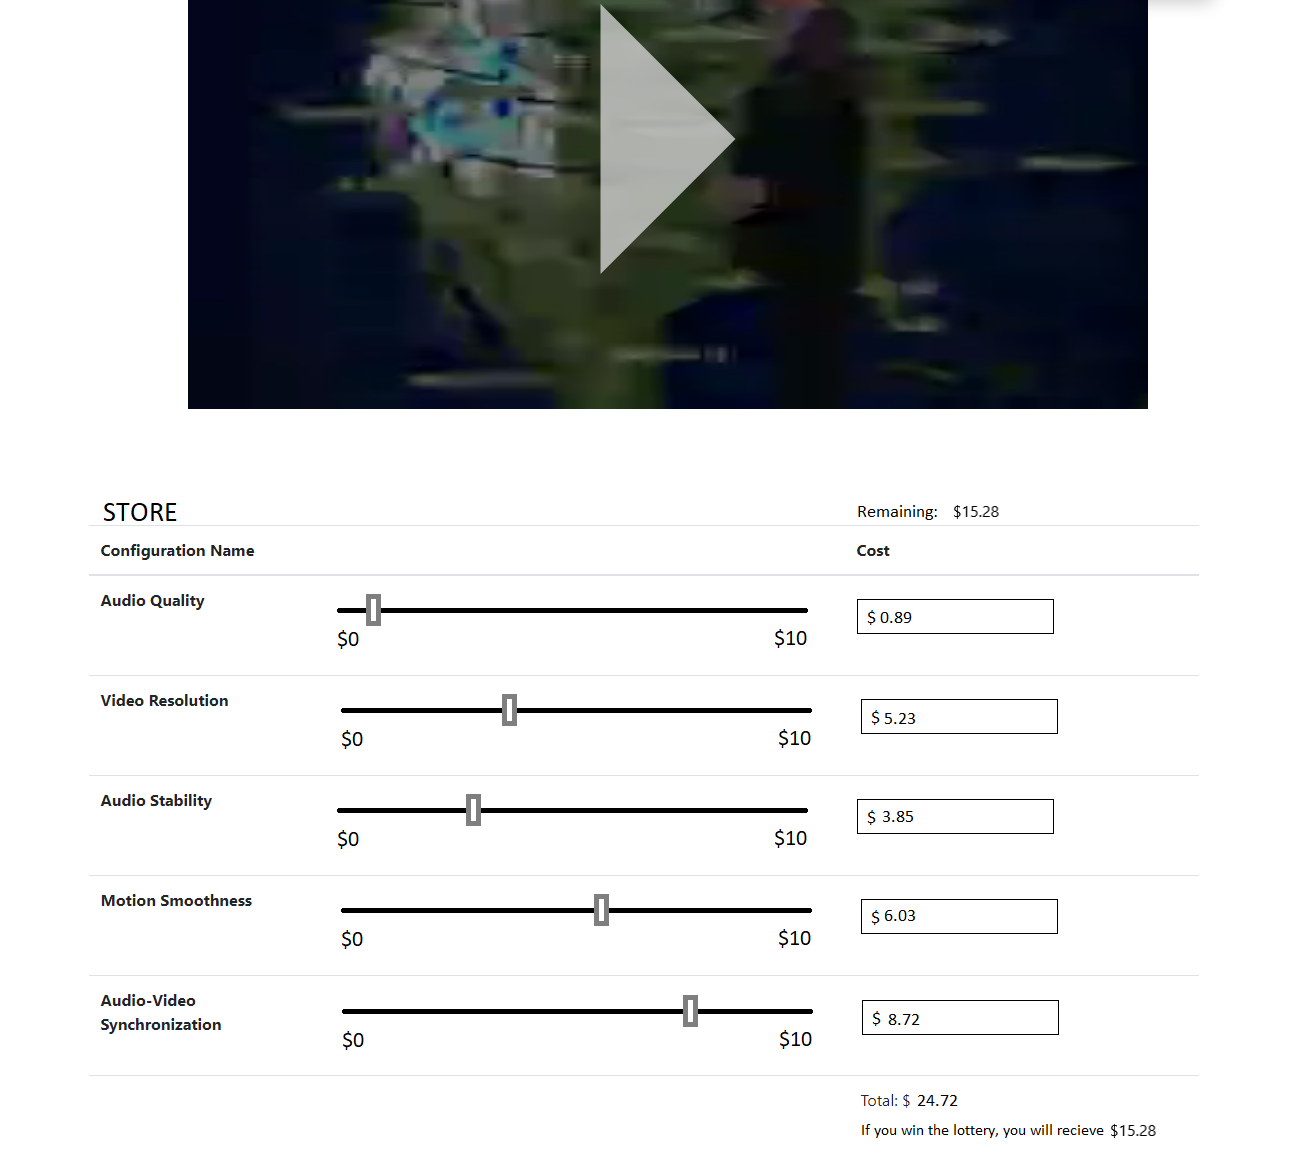
\includegraphics[width=\textwidth, keepaspectratio=true]{content/image/bb_store.png}
    \caption{
        The buyback store. This store allows participants to put in any amonut they want to spend for a particular item. The interface maps the input to a predefined level and renders the change real time.
    }
    \label{fig:exp2_store}
\end{figure}

Notice that different from the playground, the store removed the level tickers and instead provided with a slider that can stop at any location along the line. These sliders were accompanied by a text input box to the right. Participants can pull the slider anywhere, and the system would reflect the slider's relative position between 0 and 10, representing 10 dollars. Alternatively, participants can put in a value between 0 and 10, and the slider will move to the corresponding location.

These monetary value maps to one of the nine levels. When the slider moves, the video above still reflects immediately of the setting. However, participants are not aware of \textbf{how many} and \textbf{where} levels exist in this control panel. The interface will automatically translate the input value (between 0 and 10) into nine different levels. The mapping between the cost is the cost divided by 1.25. This is because there are a total of eight enhancement levels. In the case of the image, Audio Quality will be mapped to Level 0, and Video Resolution will be mapped to Level 4 and so on.

We list the nine levels here:
\begin{itemize}
    %20\%, 8\%, 4\%, and 0\%
    \item Stability of Video Imagery: 30\%, 25\%, 20\%, 12\%, 8\%, 6\%, 4\%, 2\%, and 0\%
    
    %20\%, 8\%, 4\%, and 0\%
    \item Stability of Audio: 30\%, 25\%, 20\%, 12\%, 8\%, 6\%, 4\%, 2\%, and 0\%
    
    %8kHz, 11kHz, 16kHz, and 48kHz 
    \item Quality of audio: 8kHz, 9.5kHz, 11kHz, 13kHz, 16kHz, 32kHz, 48kHz, 64khz, and 96kHz
    
    %210x280, 294x392, 364x486, and 420x560     
    \item Quality of the video: 160x214, 180x240, 210x280, 240x320, 294x392, 320x427, 364x486, 390x520, and 420x560 
    
    %1850, 1615, 1050, or 0 ms ahead
    \item Audio-Video Synchronization: 2400, 2100, 1850, 1700, 1615, 1300, 1050, 500ms or 0 ms ahead
\end{itemize}

There are several considerations for this design. One consideration is that by hiding the number of levels present, participants now have the freedom to put in any value that they ``believe'' they want to devote. The ``ticks'' do not constrain participants we presented since they do not know \textit{where} each level changes, making their input value truthful. Another consideration is that we based the nine levels on the four levels presented in the video playground. This means that we are not altering participants' previous experience, but allow them to experience and purchase more fine-grain features. The last consideration is choosing these levels based on a pilot and ensuring participants can accomplish the tasks without spending all their budgets. We detail this pilot in the appendix.

Once the participant made the purchase, the task will display a new weather forecast video. This time the control is fixed with what the participants purchased. On this page, participants can replay the video as many times as they want with the five factual multiple-choice questions on the same page. This means participants do not need to memorize the content of the video. We ask participants questions like "What is the weather of Chicago?", "What is the highs and lows of San Diego," and "Which city was not shown in the video?". These questions are similar to the ones we presented in the video playground. We also list these questions in text form to assist participants in making their purchase decisions. 

\subsection{System Design}
